%%%%%%%%%%%%%%%%%%%%%%%%%%%%%%%%%%%%%%%%%
% Beamer Presentation
% LaTeX Template
% Version 1.0 (10/11/12)
%
% This template has been downloaded from:
% http://www.LaTeXTemplates.com
%
% License:
% CC BY-NC-SA 3.0 (http://creativecommons.org/licenses/by-nc-sa/3.0/)
%
%%%%%%%%%%%%%%%%%%%%%%%%%%%%%%%%%%%%%%%%%

%----------------------------------------------------------------------------------------
%	PACKAGES AND THEMES
%----------------------------------------------------------------------------------------

\documentclass{beamer}

\mode<presentation> {

% The Beamer class comes with a number of default slide themes
% which change the colors and layouts of slides. Below this is a list
% of all the themes, uncomment each in turn to see what they look like.

%\usetheme{default}
%\usetheme{AnnArbor}
%\usetheme{Antibes}
%\usetheme{Bergen}
%\usetheme{Berkeley}
%\usetheme{Berlin}
%\usetheme{Boadilla}
%\usetheme{CambridgeUS}
%\usetheme{Copenhagen}
%\usetheme{Darmstadt}
%\usetheme{Dresden}
%\usetheme{Frankfurt}
%\usetheme{Goettingen}
%\usetheme{Hannover}
%\usetheme{Ilmenau}
%\usetheme{JuanLesPins}
%\usetheme{Luebeck}
\usetheme{Madrid}
%\usetheme{Malmoe}
%\usetheme{Marburg}
%\usetheme{Montpellier}
%\usetheme{PaloAlto}
%\usetheme{Pittsburgh}
%\usetheme{Rochester}
%\usetheme{Singapore}
%\usetheme{Szeged}
%\usetheme{Warsaw}

% As well as themes, the Beamer class has a number of color themes
% for any slide theme. Uncomment each of these in turn to see how it
% changes the colors of your current slide theme.

%\usecolortheme{albatross}
%\usecolortheme{beaver}
%\usecolortheme{beetle}
%\usecolortheme{crane}
%\usecolortheme{dolphin}
%\usecolortheme{dove}
%\usecolortheme{fly}
%\usecolortheme{lily}
%\usecolortheme{orchid}
%\usecolortheme{rose}
%\usecolortheme{seagull}
%\usecolortheme{seahorse}
%\usecolortheme{whale}
%\usecolortheme{wolverine}

%\setbeamertemplate{footline} % To remove the footer line in all slides uncomment this line
%\setbeamertemplate{footline}[page number] % To replace the footer line in all slides with a simple slide count uncomment this line

%\setbeamertemplate{navigation symbols}{} % To remove the navigation symbols from the bottom of all slides uncomment this line
}

\usepackage{graphicx} % Allows including images
\usepackage{booktabs} % Allows the use of \toprule, \midrule and \bottomrule in tables
\usepackage{listings}
\usepackage{amsmath}
\usepackage{algpseudocode,algorithm,algorithmicx}

\lstdefinestyle{customjava}{
  breaklines=true,
  frame=L,
  xleftmargin=\parindent,
  language=Java,
  showstringspaces=false,
  basicstyle=\footnotesize\ttfamily,
  keywordstyle=\bfseries\color{green!40!black},
  commentstyle=\itshape\color{gray!40!black},
  identifierstyle=\color{blue},
  stringstyle=\color{orange},
  tabsize = 2
}
%----------------------------------------------------------------------------------------
%	TITLE PAGE
%----------------------------------------------------------------------------------------

\title[Tries]{Tries} % The short title appears at the bottom of every slide, the full title is only on the title page

\author{Jonathan Windle} % Your name
\institute[UEA] % Your institution as it will appear on the bottom of every slide, may be shorthand to save space
{
University of East Anglia \\ % Your institution for the title page
\medskip
\textit{J.Windle@uea.ac.uk} % Your email address
}
\date{\today} % Date, can be changed to a custom date

\begin{document}

\begin{frame}
\titlepage % Print the title page as the first slide
\end{frame}

\begin{frame}[allowframebreaks]
\frametitle{Overview} % Table of contents slide, comment this block out to remove it
\tableofcontents % Throughout your presentation, if you choose to use \section{} and \subsection{} commands, these will automatically be printed on this slide as an overview of your presentation
\end{frame}

%------------------------------------------------------------------
\section{Intro}
\begin{frame}
\frametitle{Intro}
\begin{itemize}
\item A {\color{red}trie} t for some $S \subset K$ is a tree; either it is empty or it follows these properties:
\begin{itemize}
\item The root contains a special symbol: $\# \notin A$ 
\item Each leaf node contains a special end of key symbol: $\$ \notin A$
\item Every other node contains an element of $A$ such that:\\
$a_1a_2...a_n \in S\quad iff\quad \#a_1a_2...a_n\$$ is in path t.
\end{itemize}
\end{itemize}
\end{frame}
%---------------------------------------------------------------
\subsection{Example}
\begin{frame}
\frametitle{Example}
$A = \{
0
,
1
,
2
,
3
,
4
,
5
,
6
,
7
,
8
,
9
\}$\\
$S = \{
148
,
150
,
152
,
1523
,
1528
,
154
,
160
,
210
,
214
,
2142
,
238
,
239
\}$
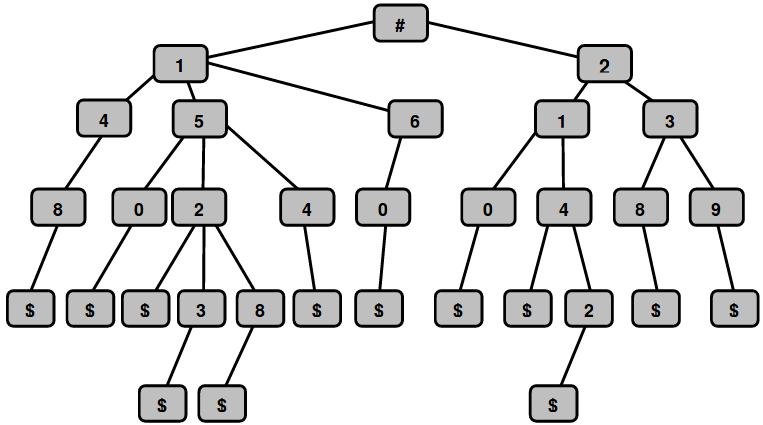
\includegraphics[scale=0.25]{example.png}
\begin{itemize}
\item Every path between the root and a leaf node corresponds to a key in $S$.
\item A trie is an appropriate representation when a combined length of all distinct prefixes in a set of keys $S$ is small compared to the total length of all keys in $S$.
\item Maximum number of children of a non-lead node is $m = |A| + 1$.
\end{itemize}
\end{frame}
%----------------------------------------------------------------
\defverbatim[colored]\lstI{
\begin{lstlisting}[style = customjava]
public class MyThread extends Thread{
	public void run(){
    	for(int i = 0; i < 13; i++)
        	System.out.println
            ("Thread Iteration " + i);
    }
}
\end{lstlisting}
}
\section{Linked list implementation}
\begin{frame}
\frametitle{Linked list implementation}
\begin{itemize}
\item First represent the trie as a binary tree:
\begin{itemize}
\item Left child in the binary tree corresponds to leftmost child in the trie.
\item Right child in the binary tree corresponds to leftmost sibling in the trie.
\end{itemize}
\item Keys are represented by character strings:
\begin{itemize}
\item The subset of characters that can be used as symbols in a key is assumed to have been specified, as is the character to be used as the end of key symbol.
\end{itemize}
\item Complexity:
\begin{itemize}
\item Search is $O(nm)$ time where $m$ is the size of the alphabet plus 1 for \$.
\item If a a branch is ``Straggly" i.e. one branch has a long branch to a single key, they can be compressed and simply go to the one coalesced key.
\end{itemize}
\end{itemize}
\end{frame}
%-----------------------------------------------------------------


\begin{frame} 
\Huge{\centerline{The End}}
\end{frame}

\end{document}